\chapter{Metodologia} \label{metodologia}

A metodologia para o desenvolvimento do compilador proposto adota uma abordagem prática, estruturada em etapas principais: a análise de informações relevantes sobre BRDFs e a compilação de \textit{shaders}; a exploração de técnicas existentes no domínio; a especificação da linguagem de entrada, um subconjunto de \LaTeX{}; a implementação do compilador; e a avaliação de seu desempenho por meio de experimentos de renderização.

Inicialmente, o método para realizar a análise e a exploração de técnicas é descrito na \autoref{analise}. Em seguida, a especificação da linguagem de entrada é apresentada na \autoref{especificacao-linguagem}. É importante destacar que a definição precisa da gramática está consolidada no capítulo de desenvolvimento, na \autoref{section-parser}.

Posteriormente, é discutida a elaboração dos casos de teste para validar a correção e a precisão do compilador, conforme detalhado na \autoref{testes}. Embora o método escolhido se baseie nesses testes iniciais, os resultados obtidos no \autoref{chapter.resultados} expandem a validação para um conjunto maior de BRDFs.

O método de implementação do compilador é detalhado na \autoref{compiladorimplementacao}, enquanto a avaliação dos experimentos de renderização, focada na qualidade visual dos \textit{shaders} compilados, é abordada na \autoref{experimentos-renderizacao}.

% A \autoref{experimentos-renderizacao} planeja o método de avaliação dos experimentos de renderização quanto a qualidade visual dos \textit{shaders} compilados.

Seguindo essa metodologia, a ferramenta proposta busca compilar descrições de BRDFs em \textit{shaders} GLSL, garantindo qualidade e precisão no resultado final.

% Posteriormente, uma ideia de como o \textit{design} dos casos de teste devem ser elaborados para validar a correção e precisão do compilador é apresentado na \autoref{testes}, apesar do metódo escolhido foi os testes que mostrando, os resultados expandem esses testes e testamos mais brdfs ainda no \autoref{chapter.resultado}. O método de implementação do compilador é detalhado na \autoref{compiladorimplementacao}. Seguindo essa metodologia, a ferramenta proposta visa compilar efetivamente descrições de BRDF em \textit{shaders} GLSL.



\section{Análise e Técnicas} \label{analise}


O primeiro passo envolve a realização de uma análise detalhada das áreas relacionadas ao desenvolvimento da ferramenta proposta. Isso inclui a revisão da literatura (\autoref{revisao}) sobre BRDFs, linguagens de \textit{shaders}, \textit{design} de compiladores e técnicas de renderização gráfica. Além disso, envolve o estudo de ferramentas e bibliotecas pertinentes.

Durante essa análise, foram estudados conceitos de radiometria para compreender tecnicamente as BRDFs. A principal fonte de informação sobre radiância e BRDFs foi o livro ``Physically Based Rendering: From Theory To Implementation'' \cite{pbr}. Esse livro foi importante para compreensão da equação de renderização (\autoref{eq-rendering-equation}).

A leitura de exemplos práticos e leitura das código fonte da ferramente \autoref{fig-disney-tool} permitiu a familiarização com o desenvolvimento de BRDFs, fornecendo uma base sólida para a compreensão do mapeamento da equação para código, aspecto fundamental para o desenvolvimento do compilador proposto neste trabalho.

Ademais, foram exploradas diversas técnicas para compilação, como o método de Pratt \textit{Parsing} para a construção de um compilador, somado ao uso do conhecimento de recursividade e caminhada em arvóres para realizar a análise semantica e geração de código.


\section{Especificação da Linguagem}\label{especificacao-linguagem}

As especificações da linguagem de entrada e saída para o compilador são definidas. A linguagem de entrada é uma versão simplificada do \LaTeX{}, na qual as expressões matemáticas nos ambientes \texttt{equation} são suficientes para descrever BRDFs. O \LaTeX{}  é um sistema de composição amplamente utilizado para documentos matemáticos e científicos. O ambiente \texttt{equation} é especificamente projetado para exibir equações individuais. O \autoref{equation-latex} é um exemplo de código-fonte \LaTeX{}  usando o ambiente \texttt{equation}.


\begin{codigo}[H]
\caption{\small Código-fonte de função quadrática.}
\label{equation-latex}
\begin{lstlisting}
\begin{equation}
    g(x) = ax^2 + bx + c
\end{equation}
\end{lstlisting}
\end{codigo}




Este código representa a equação quadrática \( g(x) = ax^2 + bx + c \), onde \( a \), \( b \) e \( c \) são coeficientes. O código GLSL correspondente gerado a partir dessa equação pode ser o \autoref{cod-glsl-g}.

\begin{codigo}[H]
\caption{\small Código GLSL da função quadrática g.}
\label{cod-glsl-g}
\begin{lstlisting}
float g(float x, float a, float b, float c) {
    return a * x * x + b * x + c;
}
\end{lstlisting}
\end{codigo}

O ambiente de equações do \LaTeX{} oferece uma ampla gama de construções matemáticas, mas, para este projeto, é necessário restringir-se a um subconjunto essencial para representar BRDFs. Ao analisar as principais BRDFs, como as citadas na \autoref{testes}, identificam-se construções indispensáveis que devem ser reconhecidas e interpretadas pelo compilador para gerar código GLSL. Estas construções são enumeradas à seguir:

\begin{enumerate}
\item Principais funções trigonométricas: \verb"\tan", \verb"\sin", \verb"\cos", \verb"\arctan", \verb"\arcsin", \verb"\arccos";
\item Função raiz quadrada: \verb"\sqrt" ($\sqrt{}$);
\item Função exponencial: \verb"\exp" ($\exp{}$);
\item Funções utilitárias: \verb"\max, \min";
\item Definições de equações, como \verb"f = x" ($f = x$);
\item Definições de funções, como \verb"f(x, y) = x^y" ($f(x, y) = x^y$);
\item Constantes comuns: \verb"\pi" ($\pi$), \verb"\epsilon" ($\epsilon$);
\item Constantes de radiometria: \verb"\theta_i" ($\theta_i$) e outras detalhadas na \autoref{tab-conventions};
\item Indicadores de vetor: \verb"\vec{}" (exemplo: $\vec{n}$);
\item Identificadores aninhados: \verb"f_{n_{i}}" ($f_{n_{i}}$);
\item Chamadas de funções: \verb"f(x+y)";
\item Operadores:
\begin{itemize}
\item Produto vetorial: \verb"x \times y" ($x \times y$);
\item Soma e Subtração: \verb"x + y", \verb"x - y";
\item Negação: \verb"-y";
\item Multiplicação: \verb"x \cdot y" ($x \cdot y$);
\item Frações: \verb"\frac{x}{y}" ($\frac{x}{y}$);
\item Divisão: \verb"x / y";
\item Potenciação: \verb"x^y" ($x^y$).
\end{itemize}
\end{enumerate}

% \label{subconjunto-latex-equantion} \begin{enumerate}
%   \item principais funções trigonometricas \verb" \tan, \sin, \cos, \arctan, \arcsin, \arccos";
%
% \item funcão raiz quadrada \verb"\sqrt" $\left(\sqrt{}\right)$;
% \item funcão exponencial \verb"\sqrt" $\left(\sqrt{}\right)$;
% \item funções utilitárias como $\max, \min$, ($\max, \min$);
% \item definição de equações, por exemplo \verb"f = x" (rederizado fica $f = x$).
% \item denifição de funções, por exemplo  \verb"f(x, y) = x^y" (rederizado fica $f(x, y) = x^y$) respectivamente;
% \item constantes comuns como \verb"\pi" ($\pi$), \verb"\epsilon" ($\epsilon$);
% \item constantes especificar \verb"\theta" ($\theta$), entre outros detalhados na @ref capitulo@;
% \item indicador de vetor como \verb"\vec{}" (ex: $\vec{n}$);
% \item identificadores aninhandos como \verb"f_{n_{i}}" ($f_{n_{i}}$).;
% \item chamada de funções \verb"f(x+y)";
% \item operadores de produto vetorial (\verb"x \times y", $x \times v$), soma ($+$), multiplicação ($x*y$ ou \verb"x \cdot y", $x \cdot y$), fração (\verb"\frac{x}{y}", $\frac{x}{y}$), divisão (\verb"{x}/{y}", ${x}/{y}$), power \verb"^", ($x^y$);
%
% \end{enumerate}

A descrição completa dos símbolos reconhecidos em nivel de código está na seção dedicado ao \textit{lexer} (\autoref{section-lexer}). A gramática completa reconhecida pelo compilador é apresentada na seção sobre o \textit{parser} (\autoref{section-parser}).

Embora o \textit{lexer} e o \textit{parser} identifiquem os símbolos, o compilador também precisa atribuir significado a eles durante a análise semântica, que ocorre após o \textit{parsing}. Por exemplo, $\omega_o$ representa o ângulo de saída da luz, enquanto $f$ é a função BRDF. Todas as convenções de símbolos suportados pela linguagem estão detalhadas na tabela \autoref{tab-conventions-metodologia}, junto com seus significados.

\begin{table}[h]
    \centering
    % \begin{tabular}{|c|l|}
    \begin{tabular}{cl}
        \hline
        \textbf{Símbolo} & \textbf{Descrição} \\
        \hline
        $\theta_i$ & Ângulo de elevação da direção da luz incidente \\
        \hline
        $\theta_o$ & Ângulo de elevação da direção da luz refletida \\
        \hline
        $\phi_i$ & Ângulo azimutal da direção da luz incidente \\
        \hline
        $\phi_o$ & Ângulo azimutal da direção da luz refletida \\
        \hline
        $\omega_i$ & Direção da luz incidente  \\
        \hline
        $\omega_o$ & Direção da luz refletida  \\
        \hline
        $f$ & BRDF de referência \\
        \hline
        $\vec{n}$ & Vetor normal à superfície \\
        \hline
        $\vec{h}$ & Vetor do meio entre $\omega_o$ e $\omega_i$ \\
        \hline
        $\theta_h$ & Ângulo entre $\vec{n}$ e $\vec{h}$ \\
        \hline
        $\theta_d$ & Ângulo entre $\omega_i$ e $\vec{h}$ \\
        \hline
    \end{tabular}
    \caption{Tabela de símbolos e suas descrições}
    \label{tab-conventions-metodologia}
\end{table}
%
%
\section{Design de Casos de Teste} \label{testes}
%
%
Os casos de teste são essenciais para validar a precisão e correção do processo de tradução do compilador. Eles estabelecem uma correspondência entre as equações \LaTeX{} de entrada, que descrevem as BRDFs, e o código de \textit{shader} GLSL esperado como saída. Um exemplo específico que demonstra a eficácia do compilador pode ser construído com a BRDF de Cook-Torrance. Sua função, \texttt{cook\_torrance}, é representada pela \autoref{eq-cook-torrance} (seu código-fonte está definido no \autoref{cod-input-latex}), onde \(D\) é a função de distribuição normal, \(G\) é a função de sombreamento geométrico e \(F\) é a função de Fresnel.

Embora as funções \(D\), \(G\), \(F\) não tenham sido definidas explicitamente, é importante ressaltar que, caso essas funções fossem definidas na equação \LaTeX{}, elas também devem ser definidas no \autoref{cod-glsl-esperado}, GLSL esperado de saída. Vale resaltar que nessa sessão de metodologia estamos dandos uma versão simplificada de como o design de casos de teste ocorre para auxiliar entendimento. Na prática, unidades, como $\rho_d$, e funções, como $D,G$ e $F$, devem estar definidas. Casos de teste completos e detalhados estão disponíveis no \autoref{chapter.resultados}.


Além disso, variáveis como a normal \( \vec{n} \) são frequentemente fornecidas como entrada para o \textit{shader} de fragmentos ou declaradas como variáveis uniformes. Por isso, elas não estão explicitamente definidas na função \texttt{cook\_torrance} do \autoref{cod-glsl-esperado}, sendo tratadas como variáveis implícitas. Uma lista completa dessas variáveis pode ser encontrada no mapeamento de convenções para código GLSL na \autoref{tab-conventions}.

Inicialmente, os casos de teste priorizam a avaliação da geração de operações e precedências. No entanto, é importante ressaltar que o compilador desenvolvido produz código GLSL que inclui a definição completa da função BRDF, juntamente com todas as variáveis de convenções necessárias. Esse código permite que a BRDF calculada seja utilizada para determinar a cor final e encaminhada para as etapas subsequentes do \textit{pipeline} gráfico, possibilitando sua renderização na ferramenta Disney BRDF Explorer.


\begin{equation} \label{eq-cook-torrance}
  \text{cook\_torrance}(\omega_i, \omega_o) = \frac{D(h)F(\omega_i, h)G(\omega_i, \omega_o, h)}{4(\omega_i \cdot n)(\omega_o \cdot n)}
\end{equation}


\begin{codigo}[H]
\caption{\small Entrada em \LaTeX\  (Cook-Torrance BRDF).}
\label{cod-input-latex}
\begin{lstlisting}
  \text{cook\_torrance}(\omega_i, \omega_o)
      = \frac{D(h)F(\omega_i, h)G(\omega_i, \omega_o, h)}{4(\omega_i \cdot n)(\omega_o \cdot n)}
\end{lstlisting}
\end{codigo}


\begin{codigo}[H]
\caption{\small Saída em GLSL esperada (Cook-Torrance BRDF).}
\label{cod-glsl-esperado}
\begin{lstlisting}[language=C]
vec3 cook_torrance(vec3 wi, vec3 wo) {
    float D_RESULT = D(h);
    vec3  F_RESULT = F(wi, wo);
    float G_RESULT = G(wi, wo, h);
    float denominador = 4.0 * dot(n, wi) * dot(n, wo);
    return D_RESULT * F_RESULT * G_RESULT / denominador;
}
\end{lstlisting}
\end{codigo}


\section{Implementação do Compilador} \label{compiladorimplementacao}

Este trabalho envolve várias tarefas-chave destinadas a completar o desenvolvimento do compilador proposto para converter equações \LaTeX{}  que descrevem BRDFs em código de \textit{shader} GLSL. As tarefas incluem: Criar um \textit{lexer} e \textit{parser} para aceitar equações \LaTeX{}; testar o \textit{lexer} para garantir o reconhecimento correto dos \textit{tokens}; testar o \textit{parser} para garantir que a árvore sintática está com precedência correta; definir símbolos predefinidos e constantes matemáticas; implementar o processo de geração de código GLSL usando a árvore sintática com o padrão de \textit{design} visitante (\textit{Visitor}); definir os casos de teste para cobrir uma certa variedade de BRDFs; testar o código gerado quanto à correção, incluindo as visualizações das BRDFs em algumas cenas.


A implementação do compilador é realizada utilizando a linguagem de programação Odin, conhecida por ser uma linguagem de propósito geral com foco em programação orientada a dados. Sua escolha se deve à sua capacidade de oferecer controle de baixo nível e a sua adequação para o desenvolvimento de sistemas complexos. Além disso, nenhuma biblioteca externa foi utilizada, sendo usada apenas as bibliotecas padrões básicas que acompanham a instalação da linguagem.

% Para a análise e construção da estrutura do compilador, foram adotadas técnicas de análise recursiva, com destaque para o método Pratt Parsing. Inicialmente, o lexer e o parser foram implementados para suportar o subconjunto da linguagem \LaTeX{} descrito em \autoref{subconjunto-latex-equantion}. O objetivo inicial foi garantir que os fundamentos do compilador estivessem funcionais, com precedências devidamente testadas na geração da árvore sintática abstrata (AST).


Para a análise e construção da estrutura do compilador, foram adotadas técnicas de análise recursiva, com destaque para o método Pratt Parsing. Inicialmente, o lexer e o parser foram implementados para suportar o subconjunto da linguagem \LaTeX{} descrito em \autoref{especificacao-linguagem}. O objetivo inicial foi garantir que os fundamentos do compilador estivessem funcionais, com precedências devidamente testadas na geração da árvore sintática abstrata (AST).

A travessia e manipulação da AST é possível pelo pacote \texttt{walker}, que abstrai operações sobre a árvore. Este pacote é utilizado em três etapas principais: adicionar parênteses para explicitar a ordem das operações, facilitando a validação; inferir recursivamente os tipos de cada expressão (nós que representam valores); e realizar a travessia da árvore com discriminação dos tipos de nós para a geração de código.

Além disso, foi implementada uma etapa de análise semântica por meio do pacote chamado \texttt{checker}. Essa etapa consiste em validar todos as expressões, criar os escopos e a tabela de símbolos, além de anotar a AST com informações como os tipos inferidos de cada nó, incluindo funções com seus domínios e contradomínios, vetores e suas dimensões, e números reais.

Por fim, com a AST devidamente anotada, foi desenvolvido o pacote \texttt{emitter}, o qual realiza a geração do código GLSL que atenda aos requisitos do pipeline gráfico. Esse código é formatado para ser carregado diretamente e renderizado na ferramenta Disney descrita na próxima seção (\autoref{disney-brdf-tool}).

\section{Experimentos de Renderização} \label{experimentos-renderizacao}


Experimentos de renderização são realizados usando os \textit{shaders} gerados pelo compilador. Isso permite a avaliação da qualidade visual das imagens renderizadas produzidas pelos \textit{shaders} compilados. A plataforma escolhida para os testes é a ferramenta \label{disney-brdf-tool} Disney BRDF Explorer \footnote{\url{https://github.com/wdas/brdf}}, compilada localmente para adicionar outros \textit{shaders}.


Essa ferramenta é composta por um renderizador e uma interface que permite ajustar parâmetros de BRDFs através de controles deslizantes em tempo real, fornecendo uma visualização interativa do efeito das mudanças nos parâmetros que afetam a aparência do objeto renderizado, como ilustrado na \autoref{fig-disney-tool}. 

O código que informa à ferramenta qual a BRDF a ser renderizada e seus possíveis parâmetros pode ser visto na \autoref{fig-disney-code}. Esse código possui um formato específico, onde se encontram algumas seções. Existe a seção para código GLSL e outra seção delimitada por \texttt{::begin parameters} e \texttt{::end parameters}, na qual podemos definir os parâmetros que se tornam constantes dessa BRDF. O nosso compilador gera shaders nesse formato.



\begin{figure}[htb]
        \caption{\label{fig-disney-tool} \small Ferramenta de visualização de BRDFs da Disney.}
        \begin{center}
            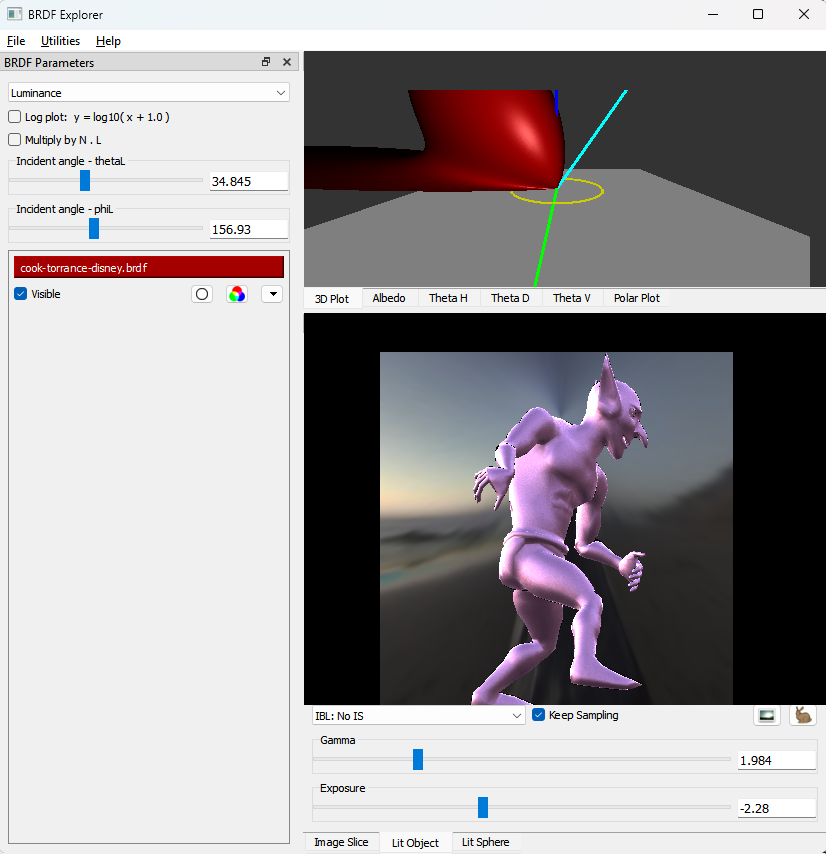
\includegraphics[scale=0.65]{./Imagens/disney-brdf-tool-original.png}
        \end{center}
  \legend{ \small Fonte: autor.}
\end{figure}


\begin{figure}[h]
        \caption{\label{fig-disney-code} \small O código GLSL com sintaxe extra para definir parâmetros.}
        \begin{center}
            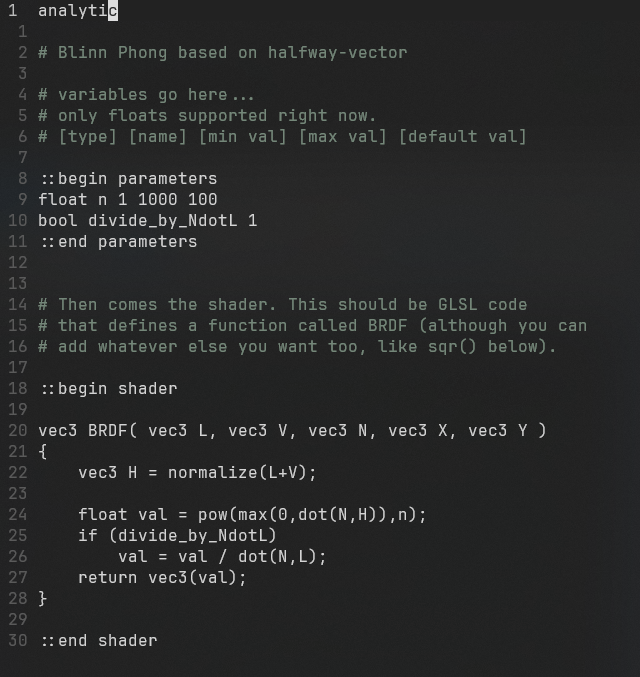
\includegraphics[scale=0.7]{./Imagens/disney-brdf-code.png}
        \end{center}
\end{figure}


